% Options for packages loaded elsewhere
% Options for packages loaded elsewhere
\PassOptionsToPackage{unicode}{hyperref}
\PassOptionsToPackage{hyphens}{url}
\PassOptionsToPackage{dvipsnames,svgnames,x11names}{xcolor}
%
\documentclass[
  letterpaper,
  DIV=11,
  numbers=noendperiod]{scrartcl}
\usepackage{xcolor}
\usepackage{amsmath,amssymb}
\setcounter{secnumdepth}{-\maxdimen} % remove section numbering
\usepackage{iftex}
\ifPDFTeX
  \usepackage[T1]{fontenc}
  \usepackage[utf8]{inputenc}
  \usepackage{textcomp} % provide euro and other symbols
\else % if luatex or xetex
  \usepackage{unicode-math} % this also loads fontspec
  \defaultfontfeatures{Scale=MatchLowercase}
  \defaultfontfeatures[\rmfamily]{Ligatures=TeX,Scale=1}
\fi
\usepackage{lmodern}
\ifPDFTeX\else
  % xetex/luatex font selection
\fi
% Use upquote if available, for straight quotes in verbatim environments
\IfFileExists{upquote.sty}{\usepackage{upquote}}{}
\IfFileExists{microtype.sty}{% use microtype if available
  \usepackage[]{microtype}
  \UseMicrotypeSet[protrusion]{basicmath} % disable protrusion for tt fonts
}{}
\makeatletter
\@ifundefined{KOMAClassName}{% if non-KOMA class
  \IfFileExists{parskip.sty}{%
    \usepackage{parskip}
  }{% else
    \setlength{\parindent}{0pt}
    \setlength{\parskip}{6pt plus 2pt minus 1pt}}
}{% if KOMA class
  \KOMAoptions{parskip=half}}
\makeatother
% Make \paragraph and \subparagraph free-standing
\makeatletter
\ifx\paragraph\undefined\else
  \let\oldparagraph\paragraph
  \renewcommand{\paragraph}{
    \@ifstar
      \xxxParagraphStar
      \xxxParagraphNoStar
  }
  \newcommand{\xxxParagraphStar}[1]{\oldparagraph*{#1}\mbox{}}
  \newcommand{\xxxParagraphNoStar}[1]{\oldparagraph{#1}\mbox{}}
\fi
\ifx\subparagraph\undefined\else
  \let\oldsubparagraph\subparagraph
  \renewcommand{\subparagraph}{
    \@ifstar
      \xxxSubParagraphStar
      \xxxSubParagraphNoStar
  }
  \newcommand{\xxxSubParagraphStar}[1]{\oldsubparagraph*{#1}\mbox{}}
  \newcommand{\xxxSubParagraphNoStar}[1]{\oldsubparagraph{#1}\mbox{}}
\fi
\makeatother

\usepackage{color}
\usepackage{fancyvrb}
\newcommand{\VerbBar}{|}
\newcommand{\VERB}{\Verb[commandchars=\\\{\}]}
\DefineVerbatimEnvironment{Highlighting}{Verbatim}{commandchars=\\\{\}}
% Add ',fontsize=\small' for more characters per line
\usepackage{framed}
\definecolor{shadecolor}{RGB}{241,243,245}
\newenvironment{Shaded}{\begin{snugshade}}{\end{snugshade}}
\newcommand{\AlertTok}[1]{\textcolor[rgb]{0.68,0.00,0.00}{#1}}
\newcommand{\AnnotationTok}[1]{\textcolor[rgb]{0.37,0.37,0.37}{#1}}
\newcommand{\AttributeTok}[1]{\textcolor[rgb]{0.40,0.45,0.13}{#1}}
\newcommand{\BaseNTok}[1]{\textcolor[rgb]{0.68,0.00,0.00}{#1}}
\newcommand{\BuiltInTok}[1]{\textcolor[rgb]{0.00,0.23,0.31}{#1}}
\newcommand{\CharTok}[1]{\textcolor[rgb]{0.13,0.47,0.30}{#1}}
\newcommand{\CommentTok}[1]{\textcolor[rgb]{0.37,0.37,0.37}{#1}}
\newcommand{\CommentVarTok}[1]{\textcolor[rgb]{0.37,0.37,0.37}{\textit{#1}}}
\newcommand{\ConstantTok}[1]{\textcolor[rgb]{0.56,0.35,0.01}{#1}}
\newcommand{\ControlFlowTok}[1]{\textcolor[rgb]{0.00,0.23,0.31}{\textbf{#1}}}
\newcommand{\DataTypeTok}[1]{\textcolor[rgb]{0.68,0.00,0.00}{#1}}
\newcommand{\DecValTok}[1]{\textcolor[rgb]{0.68,0.00,0.00}{#1}}
\newcommand{\DocumentationTok}[1]{\textcolor[rgb]{0.37,0.37,0.37}{\textit{#1}}}
\newcommand{\ErrorTok}[1]{\textcolor[rgb]{0.68,0.00,0.00}{#1}}
\newcommand{\ExtensionTok}[1]{\textcolor[rgb]{0.00,0.23,0.31}{#1}}
\newcommand{\FloatTok}[1]{\textcolor[rgb]{0.68,0.00,0.00}{#1}}
\newcommand{\FunctionTok}[1]{\textcolor[rgb]{0.28,0.35,0.67}{#1}}
\newcommand{\ImportTok}[1]{\textcolor[rgb]{0.00,0.46,0.62}{#1}}
\newcommand{\InformationTok}[1]{\textcolor[rgb]{0.37,0.37,0.37}{#1}}
\newcommand{\KeywordTok}[1]{\textcolor[rgb]{0.00,0.23,0.31}{\textbf{#1}}}
\newcommand{\NormalTok}[1]{\textcolor[rgb]{0.00,0.23,0.31}{#1}}
\newcommand{\OperatorTok}[1]{\textcolor[rgb]{0.37,0.37,0.37}{#1}}
\newcommand{\OtherTok}[1]{\textcolor[rgb]{0.00,0.23,0.31}{#1}}
\newcommand{\PreprocessorTok}[1]{\textcolor[rgb]{0.68,0.00,0.00}{#1}}
\newcommand{\RegionMarkerTok}[1]{\textcolor[rgb]{0.00,0.23,0.31}{#1}}
\newcommand{\SpecialCharTok}[1]{\textcolor[rgb]{0.37,0.37,0.37}{#1}}
\newcommand{\SpecialStringTok}[1]{\textcolor[rgb]{0.13,0.47,0.30}{#1}}
\newcommand{\StringTok}[1]{\textcolor[rgb]{0.13,0.47,0.30}{#1}}
\newcommand{\VariableTok}[1]{\textcolor[rgb]{0.07,0.07,0.07}{#1}}
\newcommand{\VerbatimStringTok}[1]{\textcolor[rgb]{0.13,0.47,0.30}{#1}}
\newcommand{\WarningTok}[1]{\textcolor[rgb]{0.37,0.37,0.37}{\textit{#1}}}

\usepackage{longtable,booktabs,array}
\usepackage{calc} % for calculating minipage widths
% Correct order of tables after \paragraph or \subparagraph
\usepackage{etoolbox}
\makeatletter
\patchcmd\longtable{\par}{\if@noskipsec\mbox{}\fi\par}{}{}
\makeatother
% Allow footnotes in longtable head/foot
\IfFileExists{footnotehyper.sty}{\usepackage{footnotehyper}}{\usepackage{footnote}}
\makesavenoteenv{longtable}
\usepackage{graphicx}
\makeatletter
\newsavebox\pandoc@box
\newcommand*\pandocbounded[1]{% scales image to fit in text height/width
  \sbox\pandoc@box{#1}%
  \Gscale@div\@tempa{\textheight}{\dimexpr\ht\pandoc@box+\dp\pandoc@box\relax}%
  \Gscale@div\@tempb{\linewidth}{\wd\pandoc@box}%
  \ifdim\@tempb\p@<\@tempa\p@\let\@tempa\@tempb\fi% select the smaller of both
  \ifdim\@tempa\p@<\p@\scalebox{\@tempa}{\usebox\pandoc@box}%
  \else\usebox{\pandoc@box}%
  \fi%
}
% Set default figure placement to htbp
\def\fps@figure{htbp}
\makeatother


% definitions for citeproc citations
\NewDocumentCommand\citeproctext{}{}
\NewDocumentCommand\citeproc{mm}{%
  \begingroup\def\citeproctext{#2}\cite{#1}\endgroup}
\makeatletter
 % allow citations to break across lines
 \let\@cite@ofmt\@firstofone
 % avoid brackets around text for \cite:
 \def\@biblabel#1{}
 \def\@cite#1#2{{#1\if@tempswa , #2\fi}}
\makeatother
\newlength{\cslhangindent}
\setlength{\cslhangindent}{1.5em}
\newlength{\csllabelwidth}
\setlength{\csllabelwidth}{3em}
\newenvironment{CSLReferences}[2] % #1 hanging-indent, #2 entry-spacing
 {\begin{list}{}{%
  \setlength{\itemindent}{0pt}
  \setlength{\leftmargin}{0pt}
  \setlength{\parsep}{0pt}
  % turn on hanging indent if param 1 is 1
  \ifodd #1
   \setlength{\leftmargin}{\cslhangindent}
   \setlength{\itemindent}{-1\cslhangindent}
  \fi
  % set entry spacing
  \setlength{\itemsep}{#2\baselineskip}}}
 {\end{list}}
\usepackage{calc}
\newcommand{\CSLBlock}[1]{\hfill\break\parbox[t]{\linewidth}{\strut\ignorespaces#1\strut}}
\newcommand{\CSLLeftMargin}[1]{\parbox[t]{\csllabelwidth}{\strut#1\strut}}
\newcommand{\CSLRightInline}[1]{\parbox[t]{\linewidth - \csllabelwidth}{\strut#1\strut}}
\newcommand{\CSLIndent}[1]{\hspace{\cslhangindent}#1}



\setlength{\emergencystretch}{3em} % prevent overfull lines

\providecommand{\tightlist}{%
  \setlength{\itemsep}{0pt}\setlength{\parskip}{0pt}}



 


\KOMAoption{captions}{tableheading}
\makeatletter
\@ifpackageloaded{caption}{}{\usepackage{caption}}
\AtBeginDocument{%
\ifdefined\contentsname
  \renewcommand*\contentsname{Table of contents}
\else
  \newcommand\contentsname{Table of contents}
\fi
\ifdefined\listfigurename
  \renewcommand*\listfigurename{List of Figures}
\else
  \newcommand\listfigurename{List of Figures}
\fi
\ifdefined\listtablename
  \renewcommand*\listtablename{List of Tables}
\else
  \newcommand\listtablename{List of Tables}
\fi
\ifdefined\figurename
  \renewcommand*\figurename{Figure}
\else
  \newcommand\figurename{Figure}
\fi
\ifdefined\tablename
  \renewcommand*\tablename{Table}
\else
  \newcommand\tablename{Table}
\fi
}
\@ifpackageloaded{float}{}{\usepackage{float}}
\floatstyle{ruled}
\@ifundefined{c@chapter}{\newfloat{codelisting}{h}{lop}}{\newfloat{codelisting}{h}{lop}[chapter]}
\floatname{codelisting}{Listing}
\newcommand*\listoflistings{\listof{codelisting}{List of Listings}}
\makeatother
\makeatletter
\makeatother
\makeatletter
\@ifpackageloaded{caption}{}{\usepackage{caption}}
\@ifpackageloaded{subcaption}{}{\usepackage{subcaption}}
\makeatother
\makeatletter
\@ifpackageloaded{fontawesome5}{}{\usepackage{fontawesome5}}
\makeatother
\usepackage{bookmark}
\IfFileExists{xurl.sty}{\usepackage{xurl}}{} % add URL line breaks if available
\urlstyle{same}
\hypersetup{
  pdftitle={ Graphs},
  pdfauthor={Arvind V.},
  colorlinks=true,
  linkcolor={blue},
  filecolor={Maroon},
  citecolor={Blue},
  urlcolor={Blue},
  pdfcreator={LaTeX via pandoc}}


\title{ Graphs}
\usepackage{etoolbox}
\makeatletter
\providecommand{\subtitle}[1]{% add subtitle to \maketitle
  \apptocmd{\@title}{\par {\large #1 \par}}{}{}
}
\makeatother
\subtitle{Charts and How they are generated from Data}
\author{Arvind V.}
\date{2021-11-01}
\begin{document}
\maketitle

\renewcommand*\contentsname{Table of contents}
{
\hypersetup{linkcolor=}
\setcounter{tocdepth}{3}
\tableofcontents
}

\begin{center}

\includegraphics[width=\linewidth,height=2.60417in,keepaspectratio]{../../../../../materials/images/2book11.jpg}
\end{center}

{````He is one of those who don't want millions, but an answer to their
questions.''}

{--- Alyosha, in The Brothers Karamazov}

\subsection{\texorpdfstring{ Setting up R
Packages}{ Setting up R Packages}}\label{setting-up-r-packages}

\begin{Shaded}
\begin{Highlighting}[]
\FunctionTok{library}\NormalTok{(tidyverse)}
\FunctionTok{library}\NormalTok{(mosaic) }\CommentTok{\# Our all{-}in{-}one package}
\FunctionTok{library}\NormalTok{(skimr) }\CommentTok{\# Looking at data}
\FunctionTok{library}\NormalTok{(ggformula) }\CommentTok{\# Our plotting package}
\FunctionTok{library}\NormalTok{(visdat) }\CommentTok{\# Mapping missing data}
\FunctionTok{library}\NormalTok{(naniar) }\CommentTok{\# Missing data visualization and munging}
\FunctionTok{library}\NormalTok{(janitor) }\CommentTok{\# Clean the data}
\FunctionTok{library}\NormalTok{(tinytable) }\CommentTok{\# Printing Tables for our data}
\FunctionTok{library}\NormalTok{(DT) }\CommentTok{\# Interactive Tables for our data}
\DocumentationTok{\#\#}
\CommentTok{\# devtools::install\_github("rpruim/Lock5withR")}
\FunctionTok{library}\NormalTok{(Lock5withR)}
\FunctionTok{library}\NormalTok{(Lock5Data) }\CommentTok{\# Some neat little datasets from a lovely textbook}
\end{Highlighting}
\end{Shaded}

\paragraph{Plot Fonts and Theme}\label{plot-fonts-and-theme}

\begin{Shaded}
\begin{Highlighting}[]
\FunctionTok{library}\NormalTok{(systemfonts)}
\FunctionTok{library}\NormalTok{(showtext)}
\DocumentationTok{\#\# Clean the slate}
\NormalTok{systemfonts}\SpecialCharTok{::}\FunctionTok{clear\_local\_fonts}\NormalTok{()}
\NormalTok{systemfonts}\SpecialCharTok{::}\FunctionTok{clear\_registry}\NormalTok{()}
\DocumentationTok{\#\#}
\FunctionTok{showtext\_opts}\NormalTok{(}\AttributeTok{dpi =} \DecValTok{96}\NormalTok{) }\CommentTok{\# set DPI for showtext}
\NormalTok{sysfonts}\SpecialCharTok{::}\FunctionTok{font\_add}\NormalTok{(}
  \AttributeTok{family =} \StringTok{"Alegreya"}\NormalTok{,}
  \AttributeTok{regular =} \StringTok{"../../../../../../fonts/Alegreya{-}Regular.ttf"}\NormalTok{,}
  \AttributeTok{bold =} \StringTok{"../../../../../../fonts/Alegreya{-}Bold.ttf"}\NormalTok{,}
  \AttributeTok{italic =} \StringTok{"../../../../../../fonts/Alegreya{-}Italic.ttf"}\NormalTok{,}
  \AttributeTok{bolditalic =} \StringTok{"../../../../../../fonts/Alegreya{-}BoldItalic.ttf"}
\NormalTok{)}

\NormalTok{sysfonts}\SpecialCharTok{::}\FunctionTok{font\_add}\NormalTok{(}
  \AttributeTok{family =} \StringTok{"Roboto Condensed"}\NormalTok{,}
  \AttributeTok{regular =} \StringTok{"../../../../../../fonts/RobotoCondensed{-}Regular.ttf"}\NormalTok{,}
  \AttributeTok{bold =} \StringTok{"../../../../../../fonts/RobotoCondensed{-}Bold.ttf"}\NormalTok{,}
  \AttributeTok{italic =} \StringTok{"../../../../../../fonts/RobotoCondensed{-}Italic.ttf"}\NormalTok{,}
  \AttributeTok{bolditalic =} \StringTok{"../../../../../../fonts/RobotoCondensed{-}BoldItalic.ttf"}
\NormalTok{)}
\FunctionTok{showtext\_auto}\NormalTok{(}\AttributeTok{enable =} \ConstantTok{TRUE}\NormalTok{) }\CommentTok{\# enable showtext}
\DocumentationTok{\#\#}
\NormalTok{theme\_custom }\OtherTok{\textless{}{-}} \ControlFlowTok{function}\NormalTok{() \{}
\NormalTok{  font }\OtherTok{\textless{}{-}} \StringTok{"Alegreya"} \CommentTok{\# assign font family up front}
  \StringTok{"\%+replace\%"} \OtherTok{\textless{}{-}}\NormalTok{ ggplot2}\SpecialCharTok{::}\StringTok{"\%+replace\%"} \CommentTok{\# nolint}

  \FunctionTok{theme\_bw}\NormalTok{(}\AttributeTok{base\_size =} \DecValTok{14}\NormalTok{, }\AttributeTok{base\_family =}\NormalTok{ font) }\SpecialCharTok{\%+replace\%} \CommentTok{\# replace elements we want to change}

    \FunctionTok{theme}\NormalTok{(}
      \AttributeTok{text =} \FunctionTok{element\_text}\NormalTok{(}\AttributeTok{family =}\NormalTok{ font), }\CommentTok{\# set base font family}

      \CommentTok{\# text elements}
      \AttributeTok{plot.title =} \FunctionTok{element\_text}\NormalTok{( }\CommentTok{\# title}
        \AttributeTok{family =}\NormalTok{ font, }\CommentTok{\# set font family}
        \AttributeTok{size =} \DecValTok{24}\NormalTok{, }\CommentTok{\# set font size}
        \AttributeTok{face =} \StringTok{"bold"}\NormalTok{, }\CommentTok{\# bold typeface}
        \AttributeTok{hjust =} \DecValTok{0}\NormalTok{, }\CommentTok{\# left align}
        \AttributeTok{margin =} \FunctionTok{margin}\NormalTok{(}\AttributeTok{t =} \DecValTok{5}\NormalTok{, }\AttributeTok{r =} \DecValTok{0}\NormalTok{, }\AttributeTok{b =} \DecValTok{5}\NormalTok{, }\AttributeTok{l =} \DecValTok{0}\NormalTok{)}
\NormalTok{      ), }\CommentTok{\# margin}
      \AttributeTok{plot.title.position =} \StringTok{"plot"}\NormalTok{,}
      \AttributeTok{plot.subtitle =} \FunctionTok{element\_text}\NormalTok{( }\CommentTok{\# subtitle}
        \AttributeTok{family =}\NormalTok{ font, }\CommentTok{\# font family}
        \AttributeTok{size =} \DecValTok{14}\NormalTok{, }\CommentTok{\# font size}
        \AttributeTok{hjust =} \DecValTok{0}\NormalTok{, }\CommentTok{\# left align}
        \AttributeTok{margin =} \FunctionTok{margin}\NormalTok{(}\AttributeTok{t =} \DecValTok{5}\NormalTok{, }\AttributeTok{r =} \DecValTok{0}\NormalTok{, }\AttributeTok{b =} \DecValTok{10}\NormalTok{, }\AttributeTok{l =} \DecValTok{0}\NormalTok{)}
\NormalTok{      ), }\CommentTok{\# margin}

      \AttributeTok{plot.caption =} \FunctionTok{element\_text}\NormalTok{( }\CommentTok{\# caption}
        \AttributeTok{family =}\NormalTok{ font, }\CommentTok{\# font family}
        \AttributeTok{size =} \DecValTok{9}\NormalTok{, }\CommentTok{\# font size}
        \AttributeTok{hjust =} \DecValTok{1}
\NormalTok{      ), }\CommentTok{\# right align}

      \AttributeTok{plot.caption.position =} \StringTok{"plot"}\NormalTok{, }\CommentTok{\# right align}

      \AttributeTok{axis.title =} \FunctionTok{element\_text}\NormalTok{( }\CommentTok{\# axis titles}
        \AttributeTok{family =} \StringTok{"Roboto Condensed"}\NormalTok{, }\CommentTok{\# font family}
        \AttributeTok{size =} \DecValTok{12}
\NormalTok{      ), }\CommentTok{\# font size}

      \AttributeTok{axis.text =} \FunctionTok{element\_text}\NormalTok{( }\CommentTok{\# axis text}
        \AttributeTok{family =} \StringTok{"Roboto Condensed"}\NormalTok{, }\CommentTok{\# font family}
        \AttributeTok{size =} \DecValTok{9}
\NormalTok{      ), }\CommentTok{\# font size}

      \AttributeTok{axis.text.x =} \FunctionTok{element\_text}\NormalTok{( }\CommentTok{\# margin for axis text}
        \AttributeTok{margin =} \FunctionTok{margin}\NormalTok{(}\DecValTok{5}\NormalTok{, }\AttributeTok{b =} \DecValTok{10}\NormalTok{)}
\NormalTok{      )}

      \CommentTok{\# since the legend often requires manual tweaking}
      \CommentTok{\# based on plot content, don\textquotesingle{}t define it here}
\NormalTok{    )}
\NormalTok{\}}

\DocumentationTok{\#\# Use available fonts in ggplot text geoms too!}
\NormalTok{ggplot2}\SpecialCharTok{::}\FunctionTok{update\_geom\_defaults}\NormalTok{(}\AttributeTok{geom =} \StringTok{"text"}\NormalTok{, }\AttributeTok{new =} \FunctionTok{list}\NormalTok{(}
  \AttributeTok{family =} \StringTok{"Roboto Condensed"}\NormalTok{,}
  \AttributeTok{face =} \StringTok{"plain"}\NormalTok{,}
  \AttributeTok{size =} \FloatTok{3.5}\NormalTok{,}
  \AttributeTok{color =} \StringTok{"\#2b2b2b"}
\NormalTok{))}
\NormalTok{ggplot2}\SpecialCharTok{::}\FunctionTok{update\_geom\_defaults}\NormalTok{(}\AttributeTok{geom =} \StringTok{"label"}\NormalTok{, }\AttributeTok{new =} \FunctionTok{list}\NormalTok{(}
  \AttributeTok{family =} \StringTok{"Roboto Condensed"}\NormalTok{,}
  \AttributeTok{face =} \StringTok{"plain"}\NormalTok{,}
  \AttributeTok{size =} \FloatTok{3.5}\NormalTok{,}
  \AttributeTok{color =} \StringTok{"\#2b2b2b"}
\NormalTok{))}

\DocumentationTok{\#\# Set the theme}
\NormalTok{ggplot2}\SpecialCharTok{::}\FunctionTok{theme\_set}\NormalTok{(}\AttributeTok{new =} \FunctionTok{theme\_custom}\NormalTok{())}
\end{Highlighting}
\end{Shaded}

\subsection{\texorpdfstring{\faIcon{chart-simple} Why
Visualize?}{ Why Visualize?}}\label{why-visualize}

\paragraph{Some Reasons}\label{some-reasons}

\begin{itemize}
\tightlist
\item
  We can digest information more easily when it is pictorial
\item
  Our
  \href{https://www.understood.org/en/articles/working-memory-what-it-is-and-how-it-works}{Working
  Memories} are both \emph{short-term} and \emph{limited} in capacity.
  So a picture abstracts the details and presents us with {an overall
  summary}, an insight, or a story that is both easy to recall and easy
  on retention.
\item
  Data Viz includes {\emph{shapes} that carry strong cultural memories};
  and impressions for us. These cultural memories help us to use data
  viz in a \emph{universal way} to appeal to a wide variety of
  audiences. {(Do humans have a gene for geometry?}\footnote{\url{https://www.xcode.in/genes-and-personality/how-genes-influence-your-math-ability/}}{)};
\item
  It helps sift facts from mere statements: for example:
\end{itemize}

\paragraph{Some Pictures}\label{some-pictures}

\begin{figure}

\begin{minipage}{0.50\linewidth}

\begin{figure}[H]

\centering{

\pandocbounded{
\includegraphics[keepaspectratio]{../../../../../materials/images/rape-capital.png}}

}

\caption{\label{fig-rape-capital}Rape Capital}

\end{figure}%

\end{minipage}%
%
\begin{minipage}{0.50\linewidth}

\begin{figure}[H]

\centering{

\pandocbounded{
\includegraphics[keepaspectratio]{../../../../../materials/images/data-reveals-crime.png}}

}

\caption{\label{fig-data_reveals-crime}Data Reveals Crime}

\end{figure}%

\end{minipage}%

\end{figure}%

\paragraph{And Finally}\label{and-finally}

\begin{itemize}
\tightlist
\item
  Visuals are a good starting point {to make \textbf{hypotheses}} of
  what may be happening in the situation represented by the data
\end{itemize}

\subsection{\texorpdfstring{ Why
Analyze?}{ Why Analyze?}}\label{why-analyze}

\paragraph{Analysis}\label{analysis}

\begin{itemize}
\tightlist
\item
  Visualizations may not tell us the true magnitude or
  {\textbf{\emph{significance}} of things}.
\item
  We need \textbf{\emph{analytic methods or statistics}} to assure
  ourselves that something is happening
\item
  These methods remove human bias and ensure that we are speaking with
  the assurance that our problem deserves.
\item
  Analysis uses {\textbf{\emph{numbers, or metrics}}}, that allow us to
  crystallize our ambiguous words/guesses.
\item
  These metrics are calculable from our data, of course, but
  \textbf{\emph{are not directly visible}}, despite often being
  intuitive.
\item
  Using these metrics, we need to become, paradoxically enough, {sure of
  our uncertainty}
\end{itemize}

So we need both visuals and analytics. And as we will see, we will not
be content with that: \emph{we will visualize our analytics, and analyze
our visualizations}!

\paragraph{What is Tidy Data?}\label{what-is-tidy-data}

Let us recall first what we meant by \textbf{\emph{tidy data}}:

\begin{figure}

\centering{


\includegraphics[width=7.08333in,height=4.16667in]{../../../../../materials/images/tidydata.jpg}

}

\caption{\label{fig-tidy-data}Tidy Data}

\end{figure}%

\paragraph{Tidy Data Principles}\label{tidy-data-principles}

\begin{itemize}
\tightlist
\item
  Each \textbf{variable} is a column;
\item
  Each column contains \emph{one kind} of data.
\item
  Each \textbf{observation} or \textbf{case} is a row.
\item
  Each \textbf{observations} contains \emph{one value} for each
  variable.
\end{itemize}

\subsection{\texorpdfstring{ What is a Data
Visualization?}{ What is a Data Visualization?}}\label{what-is-a-data-visualization}

\paragraph{\texorpdfstring{ Data Viz = Data +
Geometry}{ Data Viz = Data + Geometry}}\label{data-viz-data-geometry}

\begin{itemize}
\tightlist
\item
  How many \emph{geometric things} do we know?
\item
  Shapes? Lines? Axes? Curves? Angles? Patterns? Textures? Colours?
  Sizes? Positions? Lengths? Heights? Breadths? Radii? Textures?
\item
  All these are \textbf{geometric aspects} or \textbf{aesthetics}, each
  with \textbf{\emph{a unique property}}.
\item
  Some ``geometric things'' which we might consider are shown in the
  figure below.
\end{itemize}

\begin{figure}

\centering{

\pandocbounded{
\includegraphics[keepaspectratio]{../../../../../../content/materials/images/common-aesthetics-1.png}}

}

\caption{\label{fig-common-aesthetics}Common Geometric Aesthetics in
Charts}

\end{figure}%

\paragraph{\texorpdfstring{ Mapping}{ Mapping}}\label{mapping}

\begin{itemize}
\tightlist
\item
  How can we \textbf{\emph{manipulate}} these geometric aesthetics,
  perhaps like Kandinsky?
\item
  The aesthetic has a property, an atribute, which we can manipulate in
  accordance with a data variable!
\item
  {This act of ``mapping'' a \textbf{geometric thing} to a
  \textbf{variable} and modifying its essential property is called Data
  Visualization}
\end{itemize}

\paragraph{Mapping Examples}\label{mapping-examples}

\begin{itemize}
\tightlist
\item
  \texttt{length} or \texttt{height} of a \texttt{bar} can be made
  proportional to the\texttt{age} or \texttt{income} of a person
\item
  \texttt{Colour} of points can be mapped to \texttt{gender}, with a
  unique \texttt{colour} for each \texttt{gender}.
\item
  \texttt{Position} along an X-axis can vary in accordance with a
  \texttt{height} variable, and
\item
  \texttt{Position} along the Y-axis can vary with a \texttt{bodyWeight}
  variable.
\end{itemize}

\paragraph{Using Multiple geometries}\label{using-multiple-geometries}

\begin{itemize}
\tightlist
\item
  A chart may use more than one aesthetic: \texttt{position},
  \texttt{shape}, \texttt{colour},\texttt{height} and \texttt{angle},
  \texttt{pattern} or \texttt{texture} to name several.
\item
  Usually, each aesthetic is mapped to \textbf{just one} variable to
  ensure there is no cognitive error.
\item
  There is of course a choice and you should be able to \textbf{map} any
  kind of variable to any geometric aspect/aesthetic that may be
  available.
\end{itemize}

\paragraph{A Natural Mapping}\label{a-natural-mapping}

\begin{itemize}
\tightlist
\item
  Note that here is also a ``natural'' mapping between aesthetic and
  \textbf{kind of variable} Quantitative or Qualitative as seen in
  Figure~\ref{fig-tidy-data}.
\item
  For instance, \texttt{shape} is rarely mapped to a Quantitative
  variable;
\item
  the nature of variation between the Quantitative variable and the
  \texttt{shape} aesthetic is not similar (i.e.~not continuous).
\item
  Bad choices may lead to bad, or worse, misleading charts!
\end{itemize}

\paragraph{A Data Visualization
Example}\label{a-data-visualization-example}

\begin{Shaded}
\begin{Highlighting}[]
\FunctionTok{set.seed}\NormalTok{(}\DecValTok{1947}\NormalTok{)}
\NormalTok{diamonds }\SpecialCharTok{\%\textgreater{}\%}
  \FunctionTok{slice\_sample}\NormalTok{(}\AttributeTok{n =} \DecValTok{150}\NormalTok{, }\AttributeTok{weight\_by =}\NormalTok{ cut) }\SpecialCharTok{\%\textgreater{}\%}
  \FunctionTok{gf\_point}\NormalTok{(price }\SpecialCharTok{\textasciitilde{}}\NormalTok{ carat,}
    \AttributeTok{colour =} \SpecialCharTok{\textasciitilde{}}\NormalTok{cut,}
    \AttributeTok{shape =} \SpecialCharTok{\textasciitilde{}}\NormalTok{cut,}
    \AttributeTok{size =} \DecValTok{2}\NormalTok{, }\AttributeTok{data =}\NormalTok{ .}
\NormalTok{  ) }\SpecialCharTok{\%\textgreater{}\%}
  \FunctionTok{gf\_labs}\NormalTok{(}
    \AttributeTok{title =} \StringTok{"Plot Title = DIAMONDS ARE FOREVER"}\NormalTok{,}
    \AttributeTok{subtitle =} \StringTok{"Plot Subtitle = AND A GIRL\textquotesingle{}S BEST FRIEND"}\NormalTok{,}
    \AttributeTok{caption =} \StringTok{"Plot Caption = From the diamonds dataset"}\NormalTok{,}
    \AttributeTok{x =} \StringTok{"x{-}Axis Title = CARAT"}\NormalTok{,}
    \AttributeTok{y =} \StringTok{"y{-}Axis Title = PRICE"}
\NormalTok{  ) }\SpecialCharTok{\%\textgreater{}\%}
  \CommentTok{\# Use same name for scales to merge legends}
  \FunctionTok{gf\_refine}\NormalTok{(}
    \FunctionTok{scale\_color\_brewer}\NormalTok{(}
      \AttributeTok{name =} \StringTok{"Legend = DIAMOND QUALITY"}\NormalTok{,}
      \AttributeTok{palette =} \StringTok{"Set1"}
\NormalTok{    ),}
    \FunctionTok{scale\_shape\_manual}\NormalTok{(}
      \AttributeTok{name =} \StringTok{"Legend = DIAMOND QUALITY"}\NormalTok{,}
      \AttributeTok{values =} \FunctionTok{c}\NormalTok{(}\DecValTok{15}\SpecialCharTok{:}\DecValTok{21}\NormalTok{)}
\NormalTok{    )}
\NormalTok{  ) }\SpecialCharTok{\%\textgreater{}\%}
  \FunctionTok{gf\_annotate}\NormalTok{(}\StringTok{"text"}\NormalTok{,}
    \AttributeTok{x =} \FloatTok{1.0}\NormalTok{, }\AttributeTok{y =} \DecValTok{16000}\NormalTok{,}
    \AttributeTok{label =} \StringTok{"These DIAMONDS are}\SpecialCharTok{\textbackslash{}n}\StringTok{ Super Affordable!!"}\NormalTok{,}
    \AttributeTok{fontface =} \StringTok{"bold"}\NormalTok{,}
    \AttributeTok{size =} \FloatTok{3.5}
\NormalTok{  ) }\SpecialCharTok{\%\textgreater{}\%}
  \FunctionTok{gf\_annotate}\NormalTok{(}\StringTok{"curve"}\NormalTok{,}
    \AttributeTok{x =} \FloatTok{0.9}\NormalTok{,}
    \AttributeTok{y =} \DecValTok{14500}\NormalTok{,}
    \AttributeTok{yend =} \DecValTok{8000}\NormalTok{,}
    \AttributeTok{xend =} \FloatTok{0.95}\NormalTok{,}
    \AttributeTok{linewidth =} \DecValTok{1}\NormalTok{,}
    \AttributeTok{curvature =} \FloatTok{0.5}\NormalTok{,}
    \AttributeTok{arrow =} \FunctionTok{arrow}\NormalTok{(}\AttributeTok{length =} \FunctionTok{unit}\NormalTok{(}\FloatTok{0.5}\NormalTok{, }\StringTok{"cm"}\NormalTok{))}
\NormalTok{  ) }\SpecialCharTok{\%\textgreater{}\%}
  \FunctionTok{gf\_annotate}\NormalTok{(}
    \StringTok{"rect"}\NormalTok{,}
    \AttributeTok{xmin =} \DecValTok{1}\NormalTok{,}
    \AttributeTok{xmax =} \FloatTok{1.25}\NormalTok{,}
    \AttributeTok{ymin =} \DecValTok{2250}\NormalTok{,}
    \AttributeTok{ymax =} \DecValTok{10000}\NormalTok{,}
    \AttributeTok{alpha =} \FloatTok{0.5}\NormalTok{,}
    \AttributeTok{fill =} \StringTok{"grey80"}\NormalTok{,}
    \AttributeTok{col =} \StringTok{"black"}
\NormalTok{  ) }\SpecialCharTok{\%\textgreater{}\%}
  \FunctionTok{gf\_theme}\NormalTok{(}\FunctionTok{theme\_custom}\NormalTok{())}
\end{Highlighting}
\end{Shaded}

\begin{figure}[H]

\centering{

\pandocbounded{
\includegraphics[keepaspectratio]{index_files/figure-pdf/fig-data-vis-r-1.png}}

}

\caption{\label{fig-data-vis-r}Data Vis Components and Features}

\end{figure}%

\paragraph{What is the Mapping Here?}\label{what-is-the-mapping-here}

\begin{itemize}
\tightlist
\item
  In the above chart, it is pretty clear what kind of variable is
  plotted on the \texttt{x-axis} and the \texttt{y-axis}.
\item
  What about \texttt{colour}? Could this be considered as
  \textbf{another axis} in the chart?
\item
  There are also other aspects that you can choose (not explicitly shown
  here) such as the \texttt{plot\ theme}(colours, fonts, backgrounds
  etc)
\item
  which may \textbf{not be mapped} to data, but are nonetheless choices
  to be made.
\item
  We will get acquainted with this aspect as we build charts.
\end{itemize}

\paragraph{Transformations}\label{transformations}

\begin{itemize}
\tightlist
\item
  As we will see, Data Variables may be \textbf{\emph{transformed}}
  before being mapped to some geometric aesthetic
\item
  e.g.~we may perform \textbf{\emph{counts}} with a Qual variable that
  contains \textbf{\emph{only}} the entries \texttt{\{S,\ M,\ L,\ XL\}}.
\item
  We may also transform the \texttt{axes} (make them logarithmic, or
  even polar ) to create precisely the shape-meaning we wish. - - - This
  allows us considerable flexibility in making charts!!
\end{itemize}

\paragraph{Facets}\label{facets}

\begin{itemize}
\tightlist
\item
  Finally, if the graph is too busy, with lots of colours and shapes,
  then we can split the graph into many \textbf{small multiples} or
  \textbf{facets}, each showing a subset of the data.
\item
  This is called \textbf{faceting} and is a powerful way to reduce
  cognitive load on the viewer.
\end{itemize}

\subsection{\texorpdfstring{ Basic Types of
Charts}{ Basic Types of Charts}}\label{sec-data-viz}

\paragraph{Mapping Variables to
Aesthetics}\label{mapping-variables-to-aesthetics}

\begin{itemize}
\tightlist
\item
  We can therefore think of simple visualizations as {combinations of
  aesthetics, mapped to combinations of variables}.
\item
  It should be possible to use the many shapes we know, or can conceive
  of, and \emph{marry them to data} to create a brand new visualization
  method that advances both understanding and retention! You should
  try!!
\end{itemize}

\paragraph{Mappings and Charts: A
Catalogue}\label{mappings-and-charts-a-catalogue}

\begin{longtable}[]{@{}
  >{\raggedright\arraybackslash}p{(\linewidth - 6\tabcolsep) * \real{0.2113}}
  >{\raggedright\arraybackslash}p{(\linewidth - 6\tabcolsep) * \real{0.2113}}
  >{\raggedright\arraybackslash}p{(\linewidth - 6\tabcolsep) * \real{0.2113}}
  >{\raggedright\arraybackslash}p{(\linewidth - 6\tabcolsep) * \real{0.3662}}@{}}
\caption{Geometries , Combinations, and Graphs}\tabularnewline
\toprule\noalign{}
\begin{minipage}[b]{\linewidth}\raggedright
Variable \#1
\end{minipage} & \begin{minipage}[b]{\linewidth}\raggedright
Variable \#2
\end{minipage} & \begin{minipage}[b]{\linewidth}\raggedright
Chart Names
\end{minipage} & \begin{minipage}[b]{\linewidth}\raggedright
Chart Shape
\end{minipage} \\
\midrule\noalign{}
\endfirsthead
\toprule\noalign{}
\begin{minipage}[b]{\linewidth}\raggedright
Variable \#1
\end{minipage} & \begin{minipage}[b]{\linewidth}\raggedright
Variable \#2
\end{minipage} & \begin{minipage}[b]{\linewidth}\raggedright
Chart Names
\end{minipage} & \begin{minipage}[b]{\linewidth}\raggedright
Chart Shape
\end{minipage} \\
\midrule\noalign{}
\endhead
\bottomrule\noalign{}
\endlastfoot
Quant & None & Histogram and Density &  \\
Qual & None & Bar Chart & \\
Quant & Quant & Scatter Plot, Line Chart, Bubble Plot, Area Chart &  \\
Quant & Qual & Pie Chart, Donut Chart, Column Chart, Box-Whisker Plot,
Radar Chart, Bump Chart, Tree Diagram &  \\
Qual & Qual & Stacked Bar Chart, Mosaic Chart, Sankey, Chord Diagram,
Network Diagram &  \\
& & & \\
\end{longtable}

\subsection{\texorpdfstring{ Conclusion}{ Conclusion}}\label{conclusion}

\paragraph{Data Science Workflow}\label{data-science-workflow}

\begin{figure}

\centering{

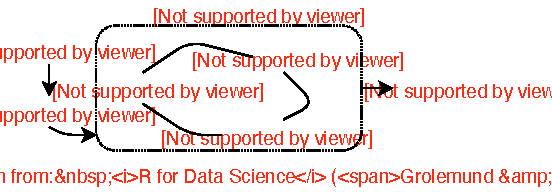
\includegraphics[width=\linewidth,height=2.5in,keepaspectratio]{index_files/mediabag/../../../../../materials/images/workflow.pdf}

}

\caption{\label{fig-datascience-workflow}Data Science Workflow}

\end{figure}%

\paragraph{Workflow Description}\label{workflow-description}

So there we have it:

\begin{itemize}
\tightlist
\item
  \textbf{\emph{Data}}: We generate data by experiment, or obtain
  readily available data. We import and clean the data
\item
  \textbf{\emph{Variables}}: Questions lead us to identify Types of
  Variables (Quant and Qual)
\item
  \textbf{\emph{Transform}}: Sometimes we may need to transform the data
  (long to wide, summarize, create new variables\ldots)
\item
  \textbf{\emph{Explore}}: Further \textbf{\emph{Questions}} lead us to
  infer \emph{relationships} between variables, the relative size of
  things, which we describe using Data Visualizations
\item
  \textbf{\emph{Report}}: This may be of interest, or best of all,
  outright surprising! Which is finally Communicated with charts and
  descriptions in a research report.
\end{itemize}

\paragraph{Grammar of Data
Visualization}\label{grammar-of-data-visualization}

You might think of all these Questions, Answers, Mapping as being
{equivalent to a grammar, as a language in itself}. And indeed, in R we
use a philosophy called the \textbf{Grammar of Graphics}! We will use
this grammar in the R graphics packages that we will encounter when we
make Graphs next. Other parts of the Workflow (Transformation,
Facetting, Analysis and Modelling) also fall within the grammar, as we
shall see.

\subsection{\texorpdfstring{ AI Generated Summary and
Podcast}{ AI Generated Summary and Podcast}}\label{ai-generated-summary-and-podcast}

\paragraph{Summary}\label{summary}

This is a tutorial on data visualization using the R programming
language. It introduces concepts such as data types, variables, and
visualization techniques. The tutorial utilizes metaphors to explain
these concepts, emphasizing the use of geometric aesthetics to represent
data. It also highlights the importance of both visual and analytic
approaches in understanding data. The tutorial then demonstrates basic
chart types, including histograms, scatterplots, and bar charts, and
discusses the ``Grammar of Graphics'' philosophy that guides data
visualization in R. The text concludes with a workflow diagram for data
science, emphasizing the iterative process of data import, cleaning,
transformation, visualization, hypothesis generation, analysis, and
communication.

\paragraph{Podcast}\label{podcast}

\subsection{\texorpdfstring{ References}{ References}}\label{references}

\begin{enumerate}
\def\labelenumi{\arabic{enumi}.}
\tightlist
\item
  Claus Wilke. \emph{Fundamentals of Data Visualization}.
  \url{https://clauswilke.com/dataviz/}
\item
  Kieran Healy. \emph{Data Visualization: A Practical Introduction}.
  \url{https://socviz.co/}
\item
  Winston Chang. \emph{R Graphics Cookbook}.
  \url{https://r-graphics.org/}
\item
  Hadley Wickham and Garrett Grolemund. \emph{R for Data Science}.
  \url{https://r4ds.had.co.nz/}
\item
  Jack Dougherty and Ilya Ilyankou. \emph{Hands-On Data Visualization}.
  \url{https://handsondataviz.org/}
\item
  Albert Rapp. \emph{Adding images to ggplot}.
  \url{https://albert-rapp.de/posts/ggplot2-tips/27_images/27_images}
\end{enumerate}

\phantomsection\label{refs}
\begin{CSLReferences}{1}{0}
\paragraph{\texorpdfstring{ R Package
Citations}{ R Package Citations}}\label{r-package-citations}

\begin{longtable}[]{@{}lll@{}}
\toprule\noalign{}
Package & Version & Citation \\
\midrule\noalign{}
\endhead
\bottomrule\noalign{}
\endlastfoot
ggformula & 0.12.2 & Kaplan and Pruim (2025) \\
Lock5Data & 3.0.0 & Lock (2021) \\
mosaic & 1.9.2 & Pruim, Kaplan, and Horton (2017) \\
TeachingDemos & 2.13 & Snow (2024) \\
\end{longtable}

\bibitem[\citeproctext]{ref-ggformula}
Kaplan, Daniel, and Randall Pruim. 2025. \emph{{ggformula}: Formula
Interface to the Grammar of Graphics}.
\url{https://doi.org/10.32614/CRAN.package.ggformula}.

\bibitem[\citeproctext]{ref-Lock5Data}
Lock, Robin. 2021. \emph{Lock5Data: Datasets for {``{Statistics:
UnLocking the Power of Data}''}}.
\url{https://doi.org/10.32614/CRAN.package.Lock5Data}.

\bibitem[\citeproctext]{ref-mosaic}
Pruim, Randall, Daniel T Kaplan, and Nicholas J Horton. 2017. {``The
Mosaic Package: Helping Students to {`{Think with Data}'} Using r.''}
\emph{The R Journal} 9 (1): 77--102.
\url{https://journal.r-project.org/archive/2017/RJ-2017-024/index.html}.

\bibitem[\citeproctext]{ref-TeachingDemos}
Snow, Greg. 2024. \emph{{TeachingDemos}: Demonstrations for Teaching and
Learning}. \url{https://doi.org/10.32614/CRAN.package.TeachingDemos}.

\end{CSLReferences}




\end{document}
